\documentclass[a4paper]{article}
\usepackage[utf8]{inputenc}
\usepackage{graphicx}
\usepackage{graphics}
\usepackage[backend=biber,style=alphabetic,]{biblatex}
\usepackage{amsmath}
\usepackage{multicol}
\usepackage{caption}
\captionsetup{
  font=small,
  labelfont=bf,
  tableposition=top
}
\usepackage{hyperref}
\usepackage{indentfirst}
\usepackage[skip=10pt plus1pt, indent=10pt]{parskip}
\usepackage[top=0.5in, bottom=0.5in, left=0.5in, right=0.5in]{geometry}
\hypersetup{
    colorlinks=true,
    linkcolor=cyan,
    citecolor=cyan,
    filecolor=magenta,
    urlcolor=cyan,
    pdftitle={Document Image Binarization},
    pdfpagemode=FullScreen,
}

\graphicspath{ {./images} }

\title{
    Document Image Binarization \\[12pt]
    \large
    ITRI617 \\[10pt]
    Prof G. Drevin \\[10pt]
    Computer Science and Information Systems \\[10pt]
    Potchefstroom Campus NWU
}
\author{Johan Venter}

\addbibresource{refs.bib}

\begin{document}

\maketitle
\newpage

\tableofcontents
\newpage
\begin{multicols}{2}
    \section{Artefact}
    The development of this artefact was inspired by the method used for document
    image binarization by~\cite{su2012robust} that is discussed later in this
    paper. This artefact takes the form of a program written in python that makes
    use of functionality from three main libraries namely
    \href{https://numpy.org/}{numpy}~\cite{numpy},
    \href{https://scikit-image.org/}{scikit-image}~\cite{scikit-image} and
    \href{https://scikit-image.org/}{scipy}~\cite{2020SciPy-NMeth} in conjunction
    with custom developed methods. \par
    A document image is provided as input where it is converted to a grayscale image for processing. It is then passed through a series of steps that each modify it in some way. The process is comprised of four main steps. The images used for testing and
    demonstration are open source, provided by
    \href{https://vc.ee.duth.gr/h-dibco2016/}{DIBCO 2016 Handwritten Document
        Dataset}.

    \noindent
    \begin{minipage}{\linewidth}
        \centering
        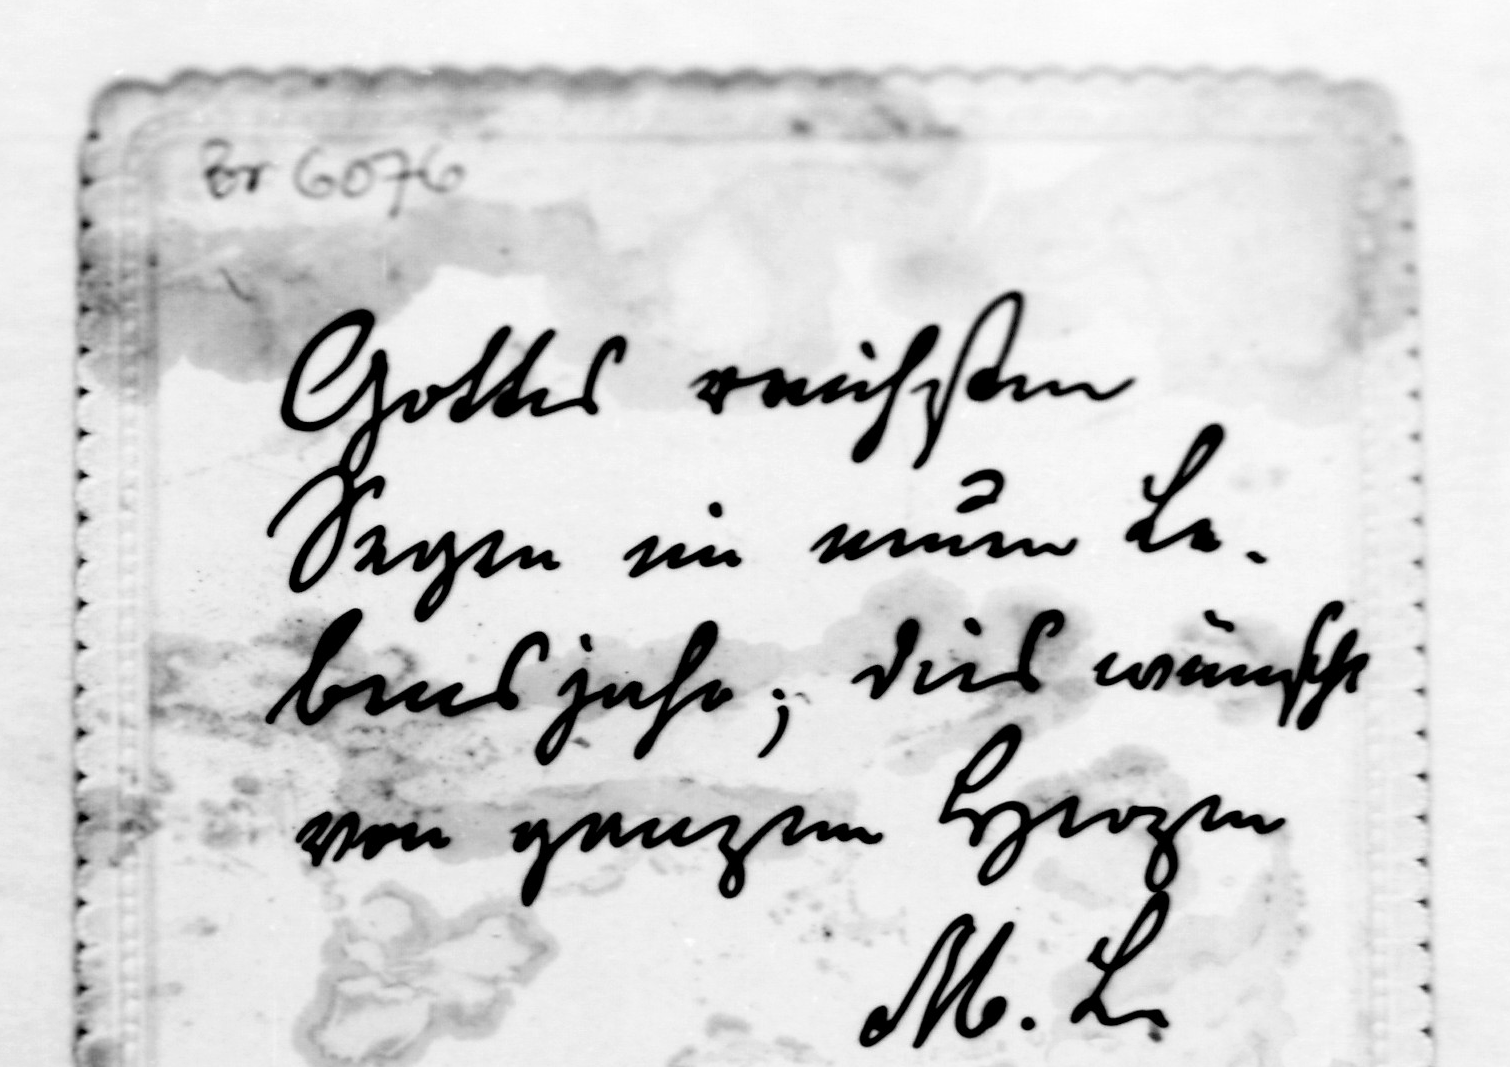
\includegraphics[width=8cm]{original.png}
        \captionof{figure}{Original Document Image}
        \label{fig:1}
    \end{minipage}

    \subsection{Denoising}
    The first step is to denoise the input document image. Both low and high freqency noise are prevalent in most images. The low freqency noise or coarse noise is filtered by  applying the wavelet denoising filter available in the scikit-image library. This filter uses the standard deviation of the intensity values of the image as an input parameter as demonstrated in Figure~\ref{fig:2}.

    \noindent
    \begin{minipage}{\linewidth}
        \centering
        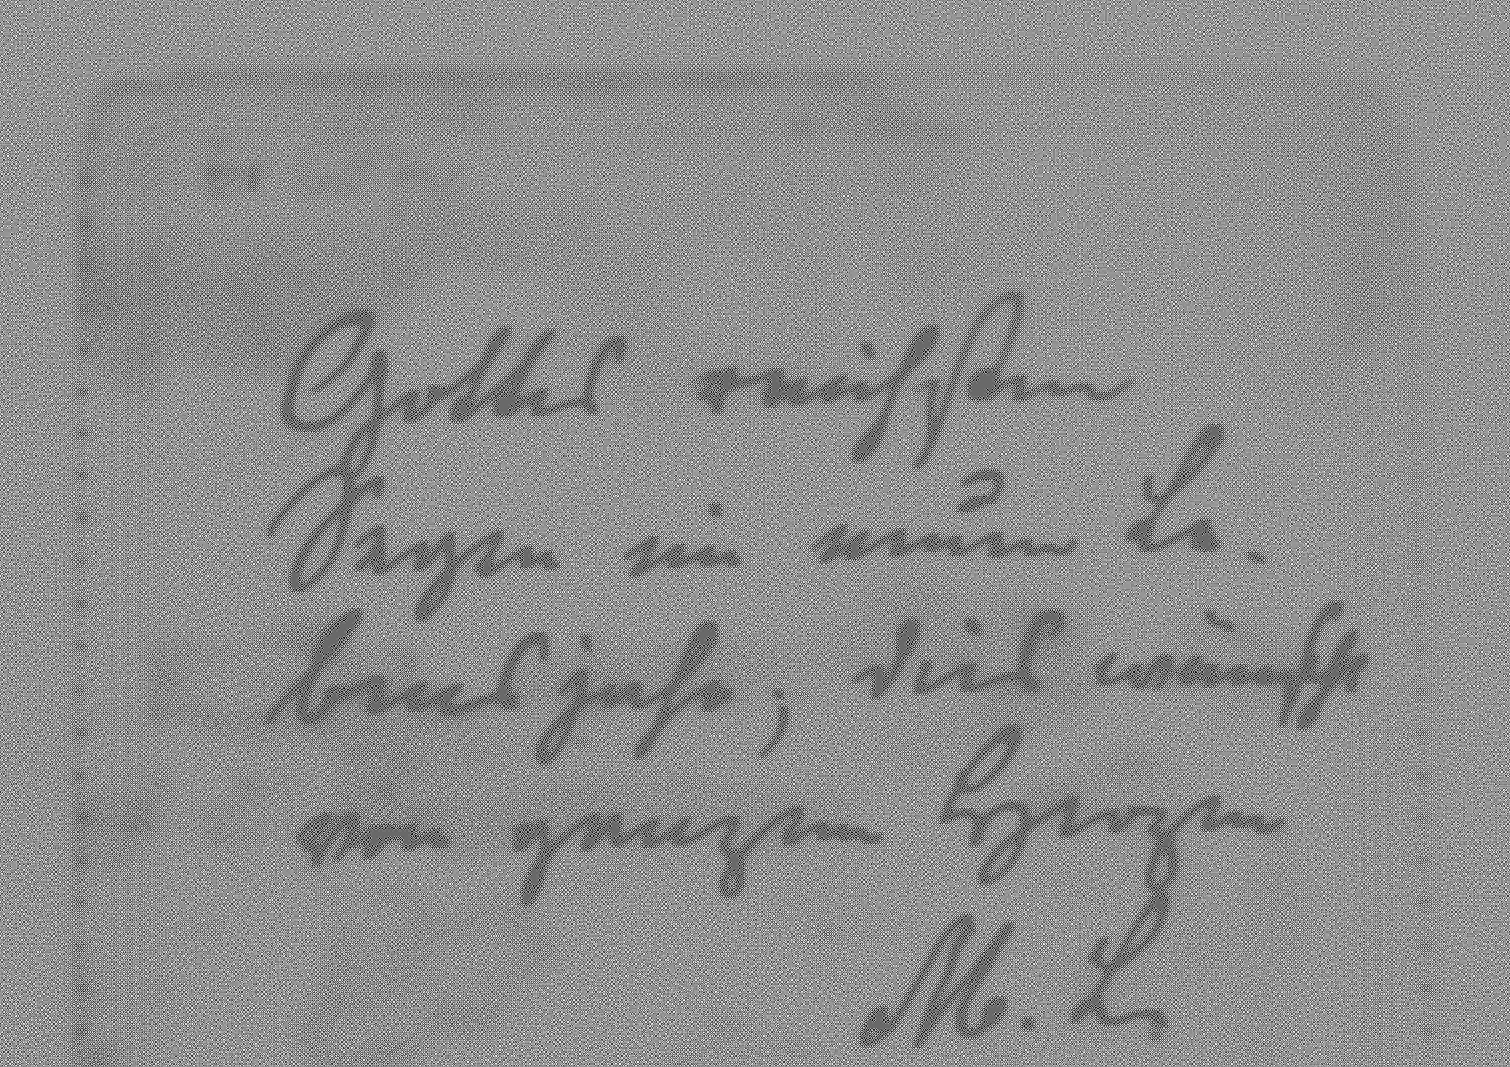
\includegraphics[width=8cm]{wavelet difference.png}
        \captionof{figure}{Noise removed by wavelet filter}
        \label{fig:2}
    \end{minipage}

    This is followed by applying a custom adaptive wiener filter that uses a 3x3 gaussian kernel for low frequency gaussian noise removal (Figure~\ref{fig:3}). At this point the image can still have gray level intensity values covering a wide range of values (it is not binarized)

    \noindent
    \begin{minipage}{\linewidth}
        \centering
        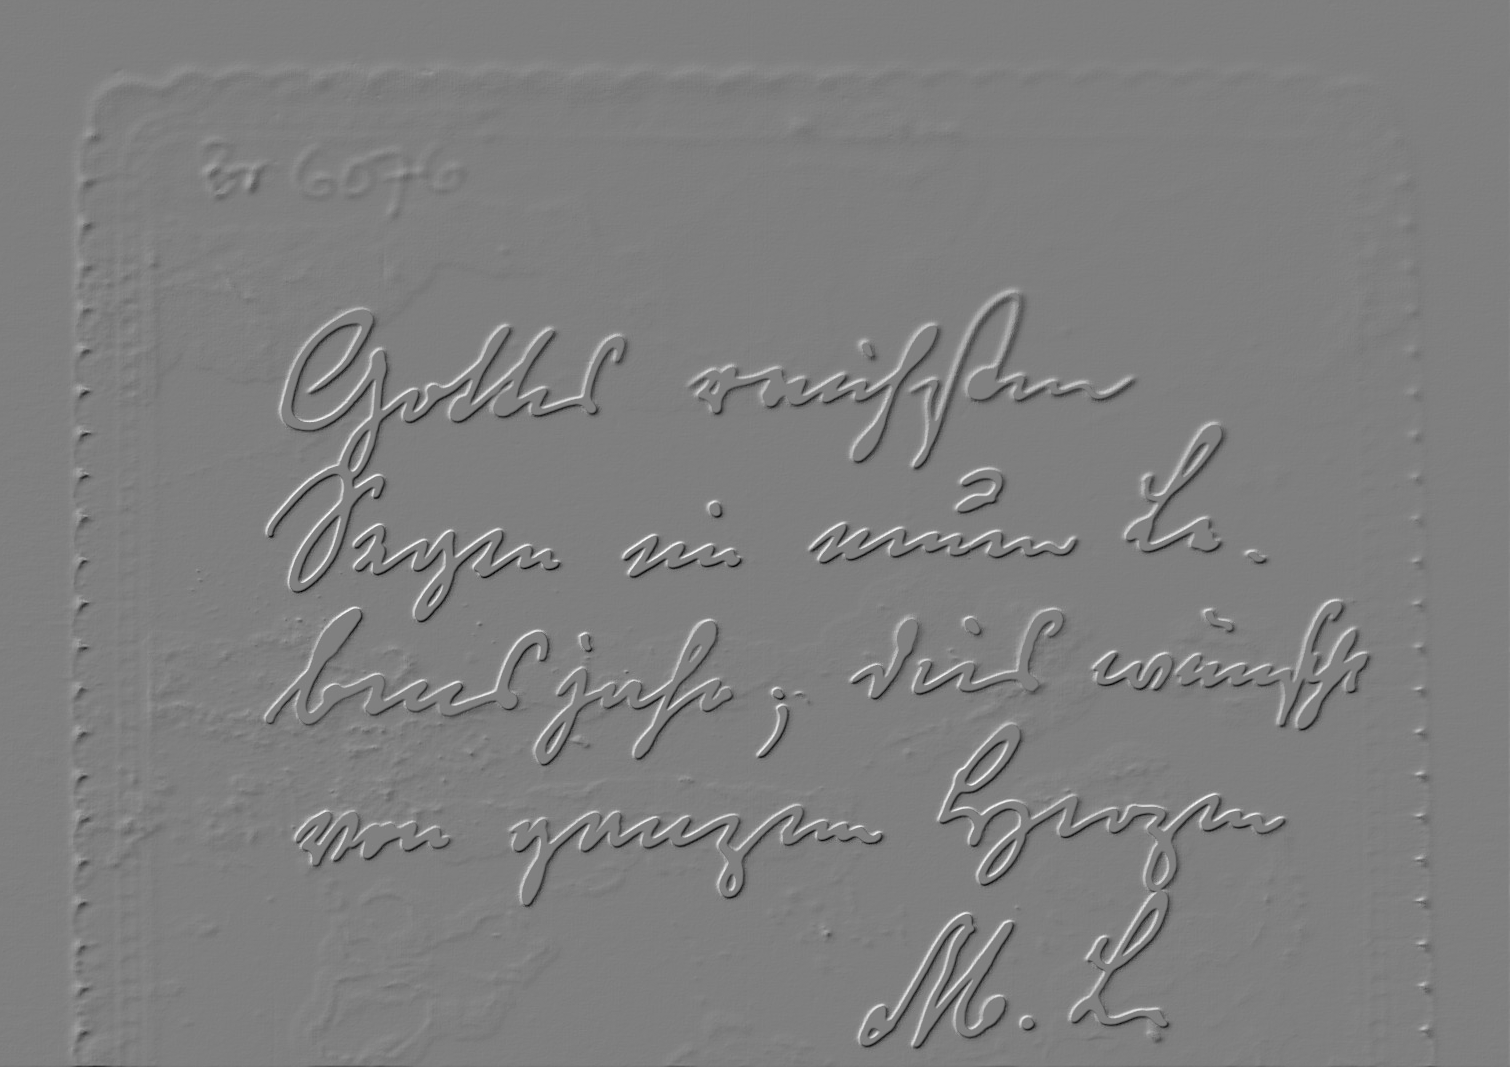
\includegraphics[width=8cm]{wiener difference.png}
        \captionof{figure}{Noise removed by wavelet filter}
        \label{fig:3}
    \end{minipage}

    \subsection{Thresholding}
    Otsu's thresholding method is used to convert the denoised image into a bi-level image (binary image / binarized image).

    \noindent
    \begin{minipage}{\linewidth}
        \centering
        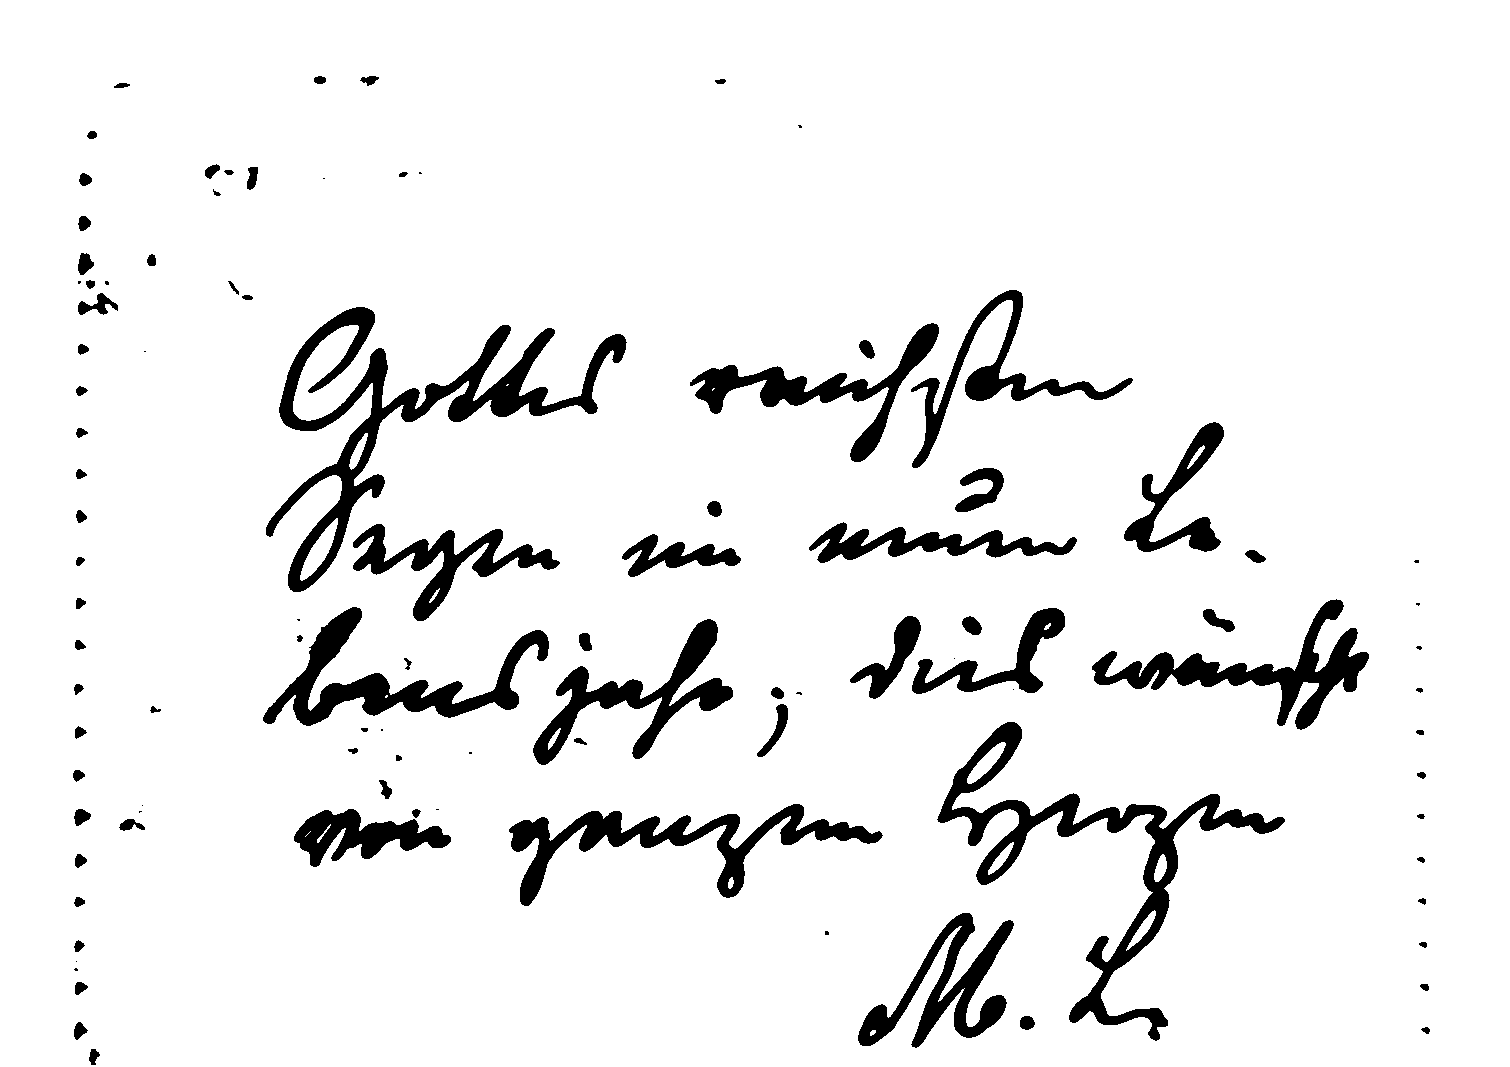
\includegraphics[width=8cm]{otsu thresholded.png}
        \captionof{figure}{Otsu thresholded image}
        \label{fig:4}
    \end{minipage}

    \subsection{Text Stroke Width Estimate}
    An estimation of text stroke width will be utilised in the final step. An effective method of doing this as introduced by~\cite{strokewidth} consists of two main steps, namely performing a distance transform and skeletonizing the image.

    \subsubsection{Distance Transform}
    The distance transform uses the thresholded image and assigns each pixel a value according to its euclidean distance to the closest white pixel (background pixel), thereby creating an image with the brightest pixels in the center of the text.

    \noindent
    \begin{minipage}{\linewidth}
        \centering
        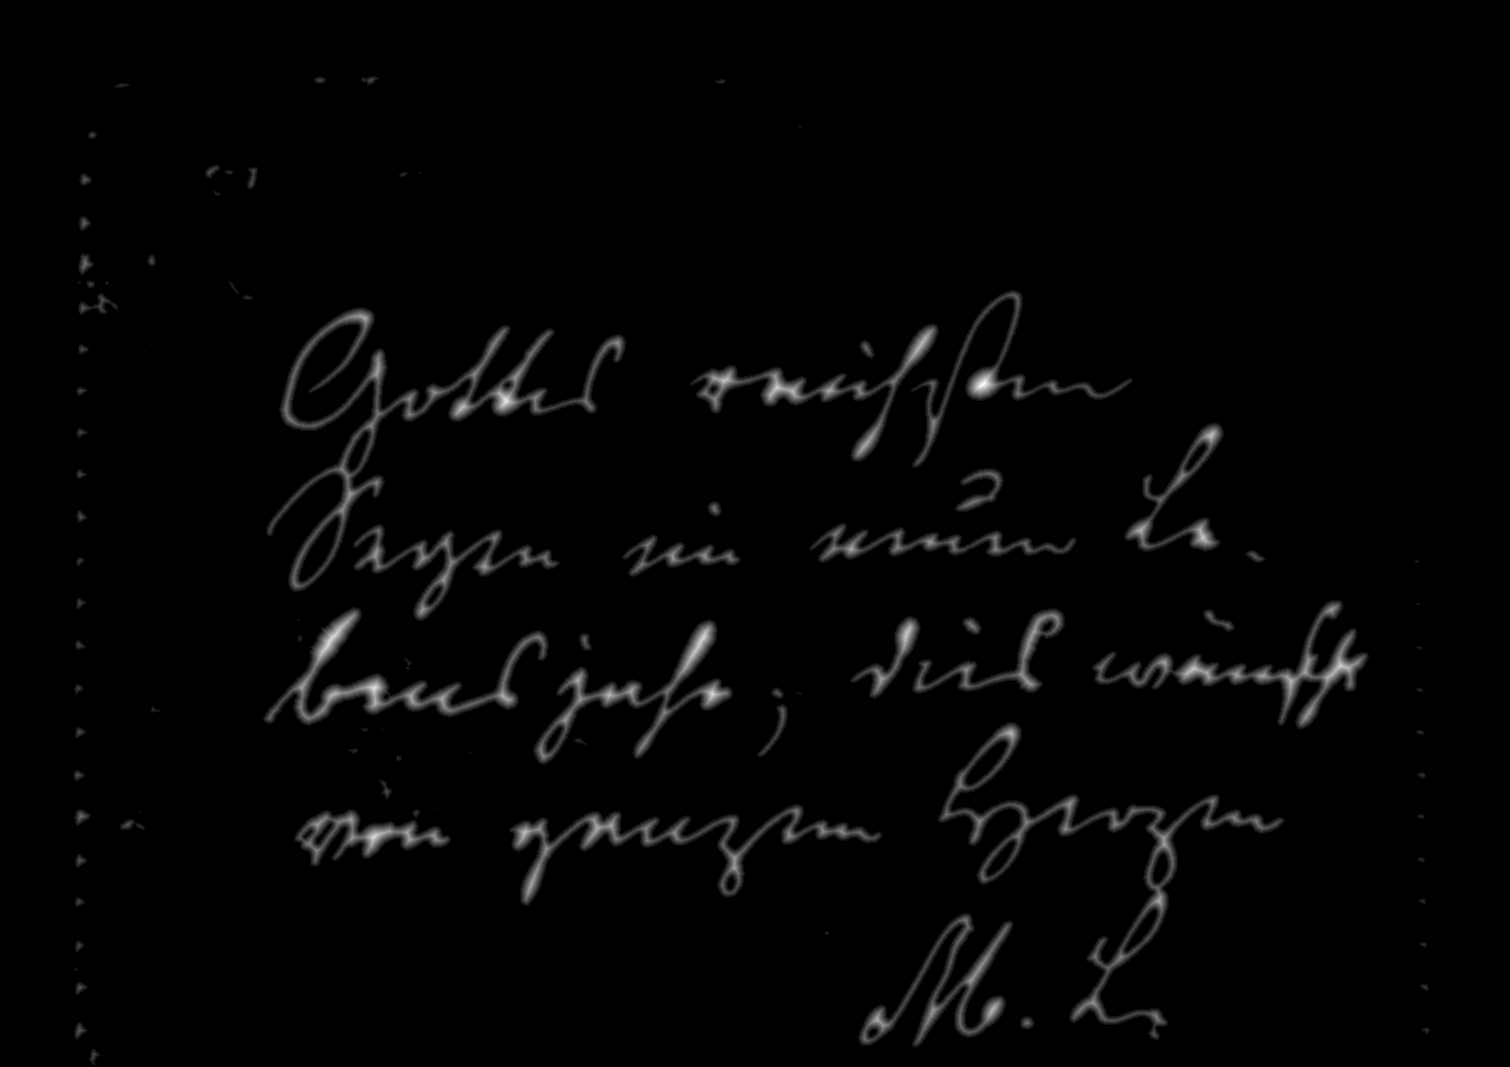
\includegraphics[width=8cm]{distance transform.png}
        \captionof{figure}{Distance transform}
        \label{fig:5}
    \end{minipage}

    \subsubsection{Skeletonizing}
    Skeletonizing an image consists of making multiple passes over an image and detecting the edge pixels. These edge pixels are then removed unless they break the connectivity of the identified object~\cite{scikit-image}.

    \noindent
    \begin{minipage}{\linewidth}
        \centering
        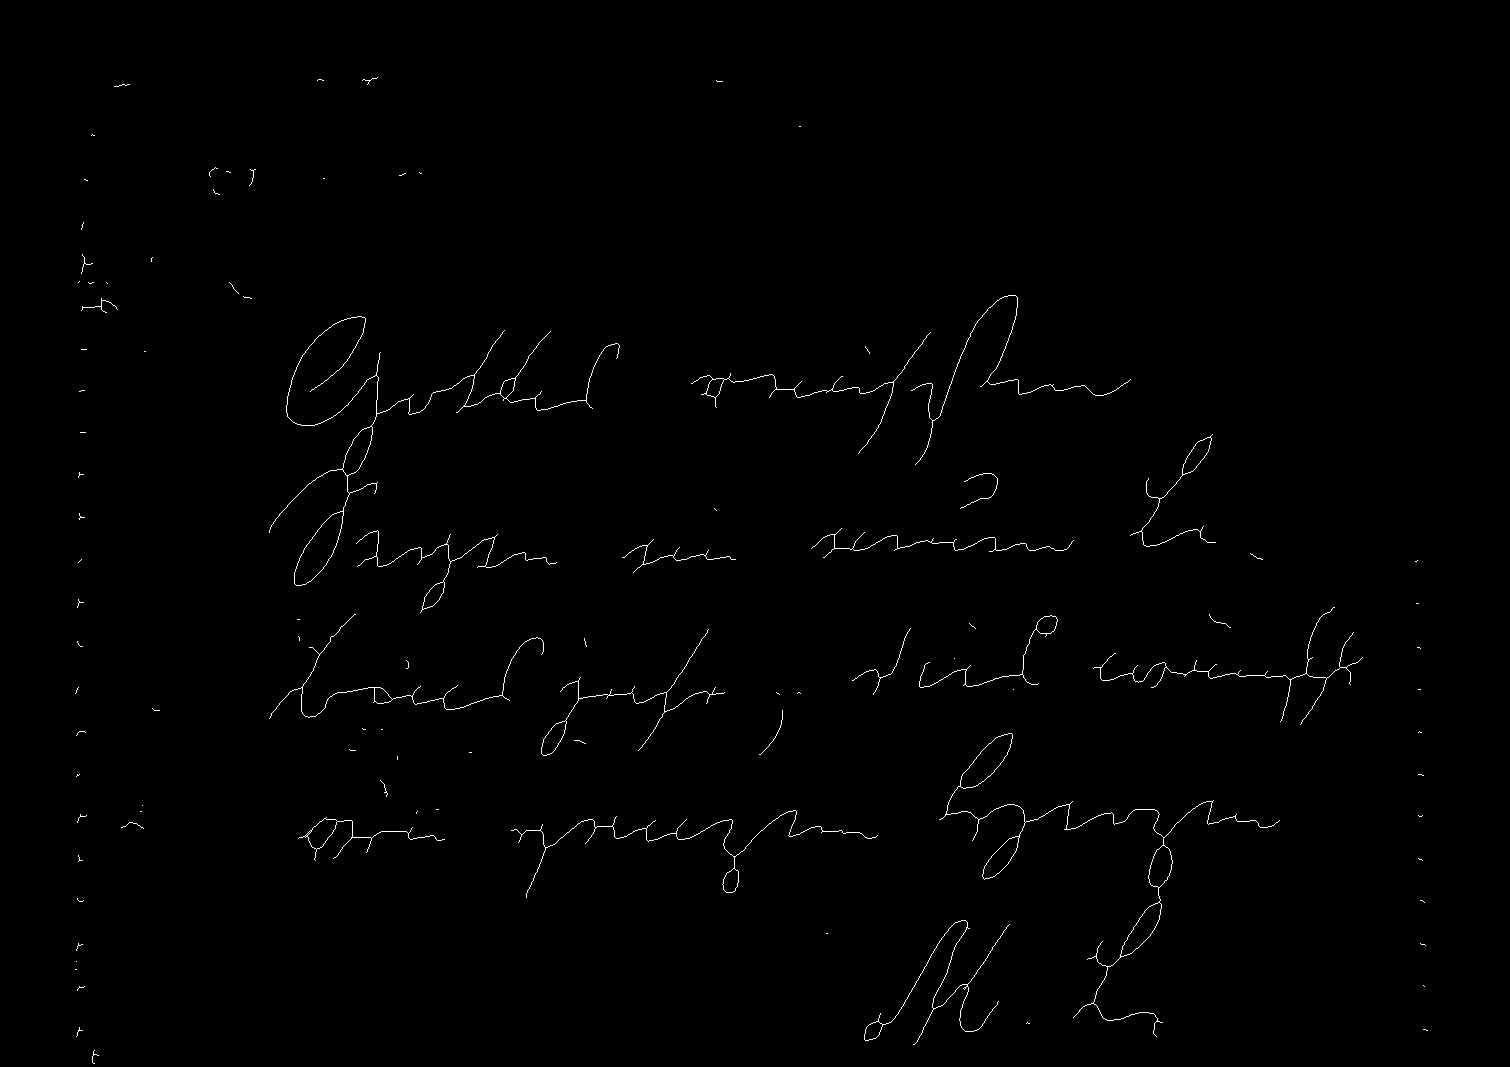
\includegraphics[width=8cm]{skeletonized.png}
        \captionof{figure}{Skeletonizing transform}
        \label{fig:6}
    \end{minipage}

    The bright pixels in the skeletonized image are then used as indexes for the selection of pixels in the distance transformed image. The selected pixel values in the distance transformed image are summed, then averaged to obtain a quantity half of the actual average text stroke width.

    \subsection{Median Filter}
    Finally, A median filter that uses the calculated stroke width as a parameter passes over the image to remove artefacts on the image smaller than the text stroke to produce the final result.

    \noindent
    \begin{minipage}{\linewidth}
        \centering
        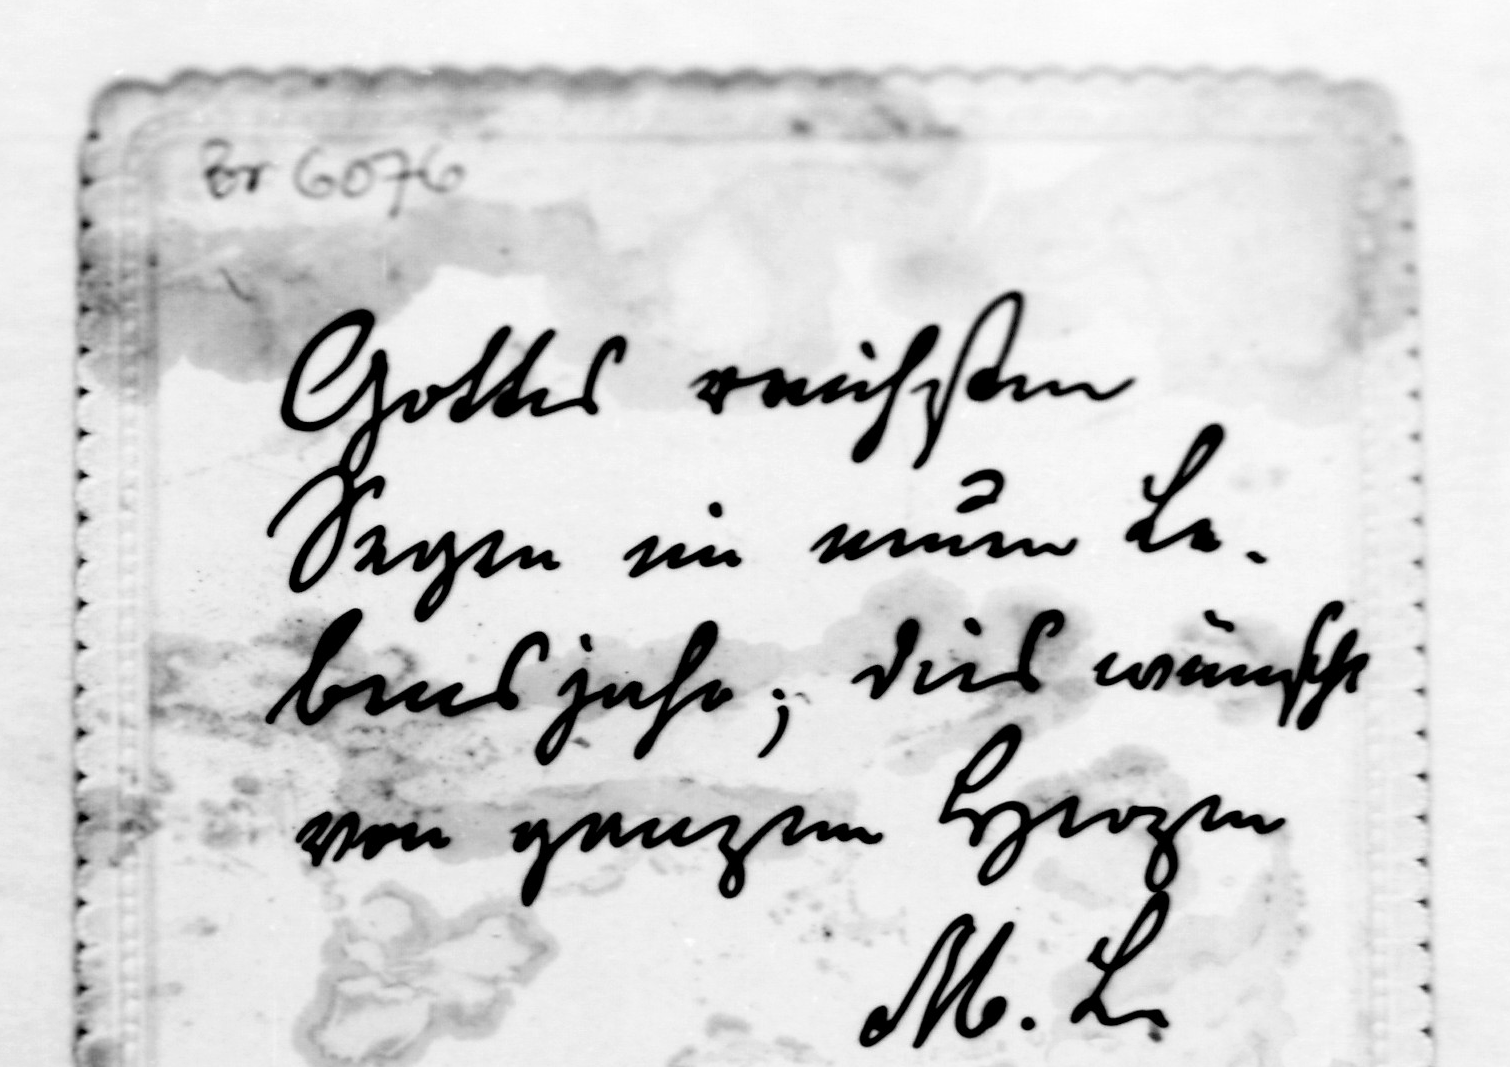
\includegraphics[width=8cm]{original.png}
        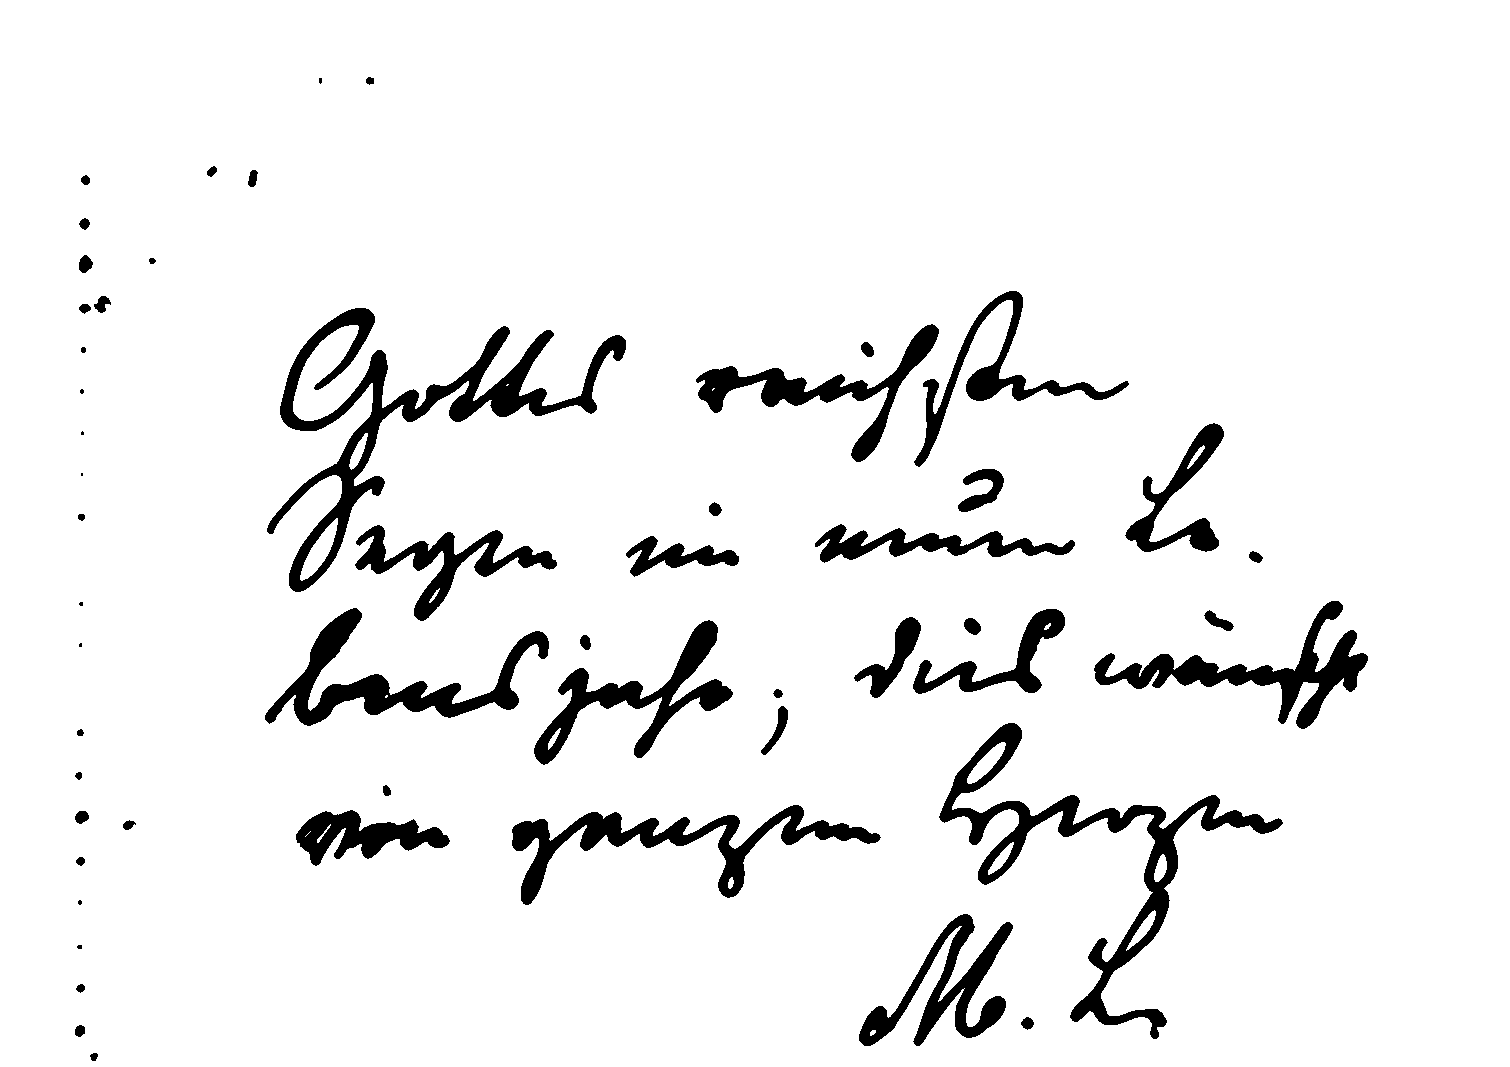
\includegraphics[width=8cm]{output.png}
        \captionof{figure}{Original vs Final Binarized Image}
        \label{fig:7}
    \end{minipage}

    \newpage

    \section{Development Lifecycle}
    The general lifecycle of the development of this project involved the iterative research and testing of multiple existing strategies.

    \subsection{Research}
    The first step in the lifecycle was the research for this project. The research needed to be directed towards gaining an understanding of the problem, the related fields and key terms and jargon related to the problems encountered.

    \subsection{Existing Solutions}
    Once a firm understanding of the field was established, existing solutions were researched and evaluated. This also required an understanding of the surrounding technologies and fundamentals of the methods used.

    \subsection{Development}
    Candidate methods, ideas and technoloies were identified and appropriate open source libraries were leveraged where needed. Several methods were implemented, tested and relinquished.

    \subsection{Iterative Approach}
    Although the main lifecycle of the development of the project was sequential, each step happened iteratively.

    \section{Development of the Artefact}
    As a guide for methods relating specifically to document image binarization, two main sources were utilised~\cite{su2012robust}~\cite{gatos2006adaptive}. For general image processing principles and practices \href{https://numpy.org/}{numpy}~\cite{numpy},
    \href{https://scikit-image.org/}{scikit-image}~\cite{scikit-image} and
    \href{https://scikit-image.org/}{scipy}~\cite{2020SciPy-NMeth} were invaluable.

    \subsection{Denoising}
    \subsubsection{Wiener Filter}
    The Wiener filter is optimal by the mean squared error measure, since it is defined by it. This property along with popular use and consistency of results by ~\cite{6524379}, ~\cite{gatos2006adaptive} makes the wiener filter as well as wavelet filters the obvious choice as candidates for denoising the document images.
    \par
    ~\cite{gatos2006adaptive} describes the use of an adaptive wiener filter that makes use of the local properties in an image to reduce noise using the following formula:
    \[I(x,y)=\mu+\frac{(\sigma^2-v^2)(I_{source}-\mu)}{\sigma^2}\]
    where \(\mu\) is the local mean, \(\sigma^2\) the variance in a 3 x 3 window and \(v^2\) is the average variance.
    \par
    The selected algorithm is a variation on the original Wiener filter, called the Wiener-Hunt filter that transforms the image into the freqency domain first by using the fourier transform
    \[\hat x = F^\dagger (|\Lambda_H|^2 + \lambda |\Lambda_D|^2)
        \Lambda_H^\dagger F y\]
    with \(F\) and \(F^\dagger\) the Fourier and inverse Fourier transforms respectively, \(\Lambda_H\) the Fourier transform of the transfer function and \(\lambda\) a damping constant as described by~\cite{scikit-image}.

    \subsubsection{Wavelet Filter}
    The wavelet transform decomposes the image into a collection of wavelets. A wavelet is a wave-like function, that has a finite 'energy' and symmetric area around the x-axis. The transform can be interpreted as the convolution of a set of wavelets over the image that will output a signal proportional to the similarity between the wavelets and the image.
    \[ \int_{-\infty}^{\infty} f(x,y) \cdot g(x,y) \,dx \]

    \par
    Other Denoising methods were considered such as total variation denoising and bilateral denoising.

    \subsection{Thresholding}

    % \subsection{Gradient Image}
    % An image is constructed using a formula for identifying local image contrast:
    % \begin{equation}
    %     \label{E:1}
    %     C(i,j)=\frac{I_{max}(i,j)-I_{min}(i,j)}{I_{max}(i,j)+I_{min}(i,j)+\epsilon}
    % \end{equation}
    % where \(\epsilon\) is a positive infinitesimal. The denominator scales the input according to the local range of values, thereby normalizing the contrast across the image~\cite{su2012robust}. Next, a constant \(a\) is calculated:
    % \begin{equation}
    %     \label{E:2}
    %     a=(\frac{\sigma}{128})^\gamma, \; \gamma \geq 0
    % \end{equation}
    % \(\sigma\) is the standard deviation of the entire document image intensities.
    % By combining \ref{E:1} and \ref{E:2} we derive the final equation they use to construct the Gradient image:
    % \begin{equation}
    %     \label{E:3}
    %     C_a(i,j)=a\times C(i,j)+(1-a)(I_{max}(i,j)-I_{min}(i,j))
    % \end{equation}
    % Which results in
    % \begin{figure}[htp]
    %     \centering
    %     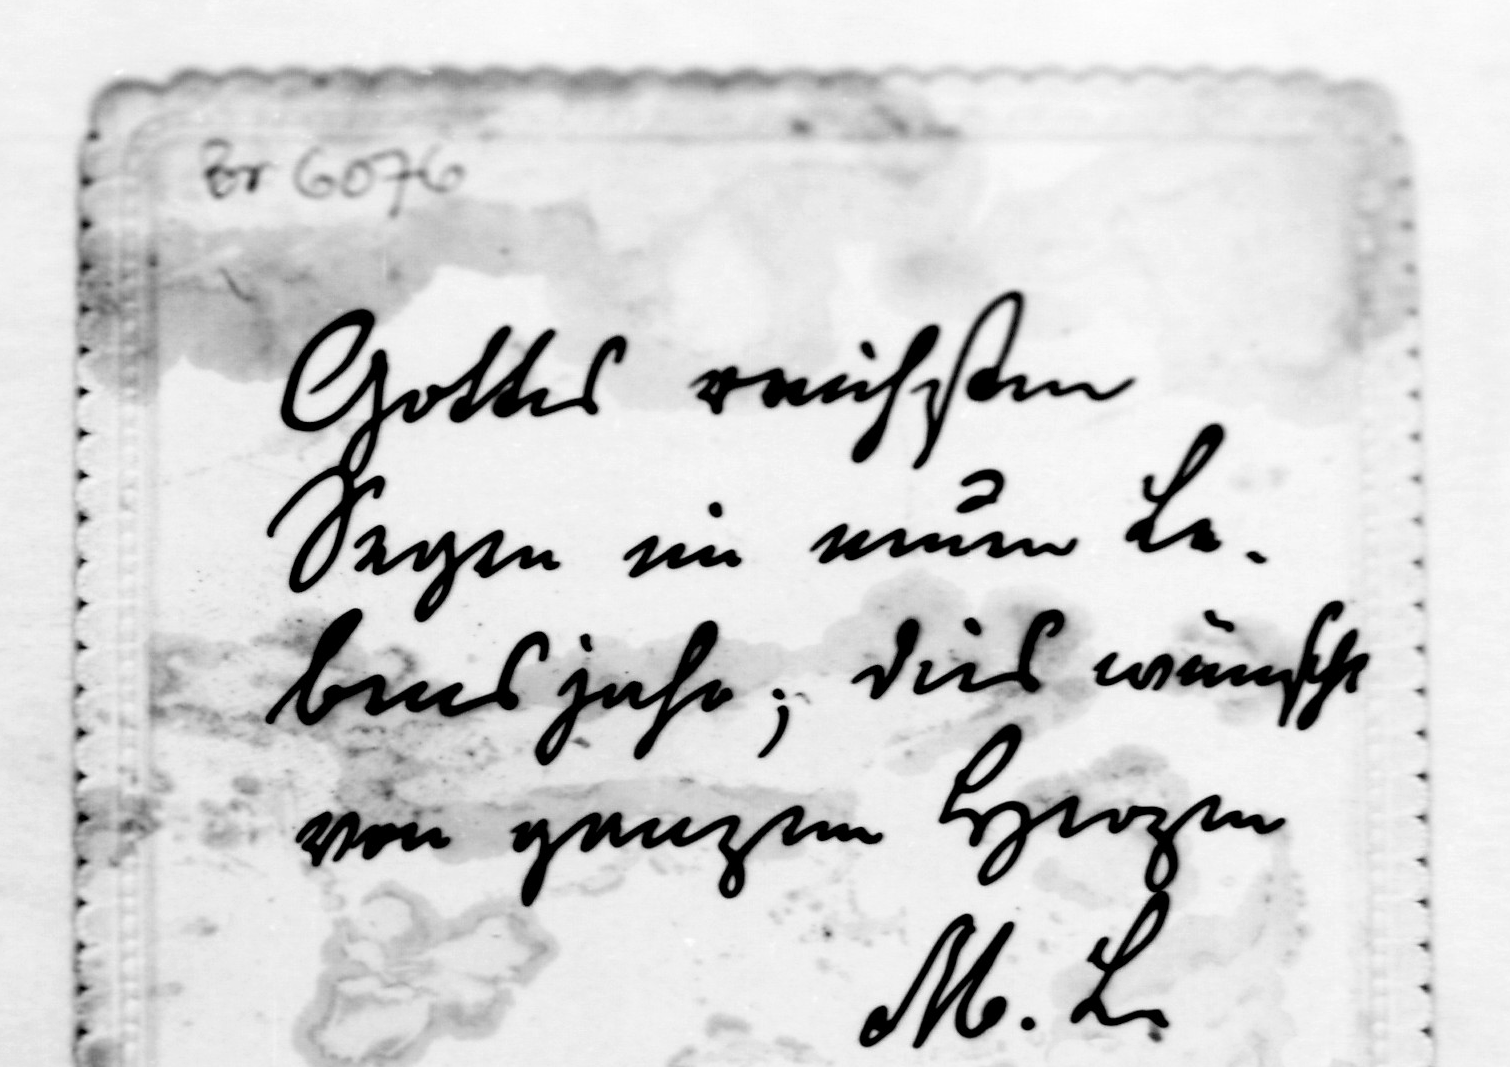
\includegraphics[width=4cm]{original.png}
    %     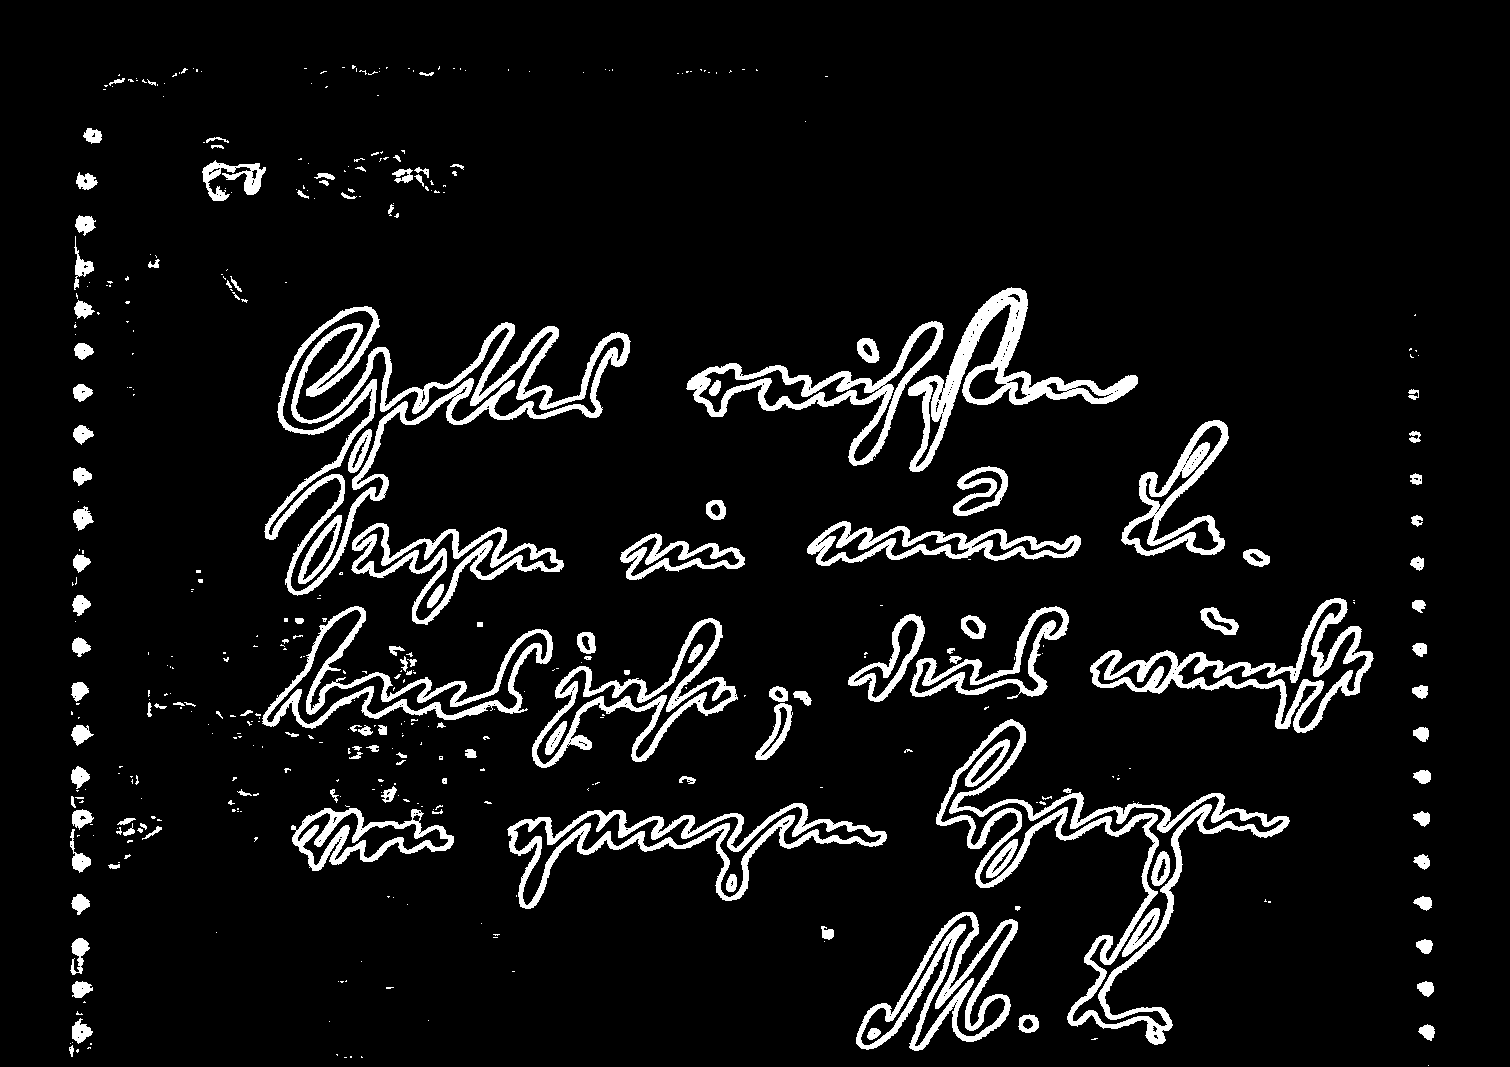
\includegraphics[width=4cm]{contrast-image.png}
    %     \caption{Original Document Image and Contrast Image}
    %     \label{fig:7}
    % \end{figure}

    % \subsection{Thresholding}

    \newpage
    \printbibliography
\end{multicols}
\end{document}